\subsection{Solution of ideal dipole problem}

\begin{frame}{Solution of ideal dipole problem}
    \begin{columns}
        \column{0.4\textwidth}
        \vspace{-4mm}
        
        With \( \beta = \omega/c \), \( \eta = \sqrt{\mu/\varepsilon}\) \\
        
        \vspace{2mm}
        
        The vector Potential is
        \begin{align*}
            \mathbf{A} & = \iiint_{v'} \mu \mathbf{J} \dfrac{ \exp( - j \beta R ) }{ 4 \pi R } \mathrm{d} v' \\
            & = \dfrac{ \mu I \exp( - j \beta r ) }{ 4 \pi R} L \mathbf{\hat{z}}.
        \end{align*}

        \begin{itemize}
            \item Magnetic fields:
        \end{itemize}
        \begin{equation*}
            \mathbf{H} = \dfrac{1}{\mu} \nabla \times \mathbf{A}.
        \end{equation*}

        \begin{itemize}
            \item Electric fields:
        \end{itemize}
        \begin{equation*}
            \mathbf{E} = \dfrac{1}{j \omega \epsilon} \nabla \times \mathbf{H}.
        \end{equation*}
        
        \column{0.6\textwidth}
        \vspace{-4mm}
        \begin{equation*}
            I(z') = \left\{
            \begin{array}{ll}
                I_0 & x'=0, y'=0, \lvert z' \rvert \le L/2.  \\
                0 & \text{everywhere else}.
            \end{array}
            \right.
        \end{equation*}
        
        \begin{figure}
            \centering
            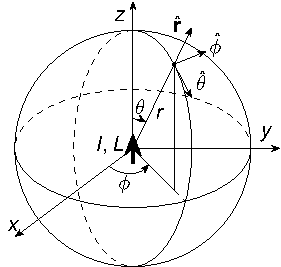
\includegraphics[width=0.7\textwidth]{Figures/Dipole_in_sphere_coordinate.pdf}
            \caption{Ideal dipole in sphere coordinate.}
            \label{fig:Ideal_dipole}
        \end{figure}
    \end{columns}
\end{frame}

%% Slide 2

\begin{frame}{Solution of ideal dipole problem}

    \vspace{-6mm}
    
    \begin{align*}
        \mathbf{A} = & \dfrac{\mu I \exp (-j \beta r)}{4 \pi r} L \mathbf{\hat{z}}, \\
        & \\
        \mathbf{H} = & \dfrac{I L}{4\pi} j \beta \left( 1 + \dfrac{1}{j \beta r} \right) \dfrac{ \exp ( - j \beta r) }{r} \sin \theta \mathbf{ \hat{\phi} }, \\
        & \\
        \mathbf{E} = & \dfrac{I L}{4\pi} j \omega \mu \left[ 1 + \dfrac{1}{j \beta r} - \dfrac{1}{(\beta r)^2} \right] \dfrac{ \exp ( - j \beta r) }{r} \sin \theta \mathbf{ \hat{\theta} } \\
        &+ \dfrac{I L}{2\pi} \eta \left[ \dfrac{1}{r} - j \dfrac{1}{\beta r^2} \right] \dfrac{ \exp ( - j \beta r) }{r} \cos \theta \mathbf{ \hat{r} }, \\
        & \\
        \mathbf{S} = & \dfrac{1}{2} \mathbf{E} \times \mathbf{H}^*.
    \end{align*}
\end{frame}